\documentclass[11pt]{article}
\usepackage[T1]{fontenc}
\usepackage{lmodern}
\usepackage{parskip}
\usepackage[colorlinks=true,urlcolor=Blue,linkcolor=black,citecolor=black]{hyperref}
\usepackage{graphicx}
\usepackage{amsmath}
\usepackage[utf8]{inputenc}
\usepackage[spanish]{babel}
\usepackage{fancyhdr}
\usepackage{csquotes}
\usepackage{lastpage}
\usepackage{array}
\usepackage{listings}
\usepackage{color}
\definecolor{dkgreen}{rgb}{0,0.6,0}
\definecolor{gray}{rgb}{0.5,0.5,0.5}
\definecolor{mauve}{rgb}{0.58,0,0.82}
\usepackage[affil-it]{authblk}
\usepackage[activate={true,nocompatibility},final,tracking=true,kerning=true,spacing=true,factor=1100,stretch=10,shrink=10]{microtype}
\usepackage[hmargin=2cm,top=4cm,headheight=65pt,footskip=65pt]{geometry}
\usepackage{hyperref}
\usepackage{graphicx}
\usepackage{float}
\graphicspath{ {./screenshots/p03/} }

% Documento
\begin{document}

% Título
\title{IFA. Práctica de laboratorio 03}

\author{Hugo Fonseca Díaz \\ email \href{mailto:uo258318@uniovi.es}{uo258318@uniovi.es}}
\affil{Escuela de Ingeniería Informática. Universidad de Oviedo.}

\maketitle

% Ejercicio 1
\section{Ejercicio 1}
Se crea el caso en Autopsy con los datos solicitados.

\begin{figure}[H]
  \caption{Ejercicio 1: Creación del caso}
  \centering
  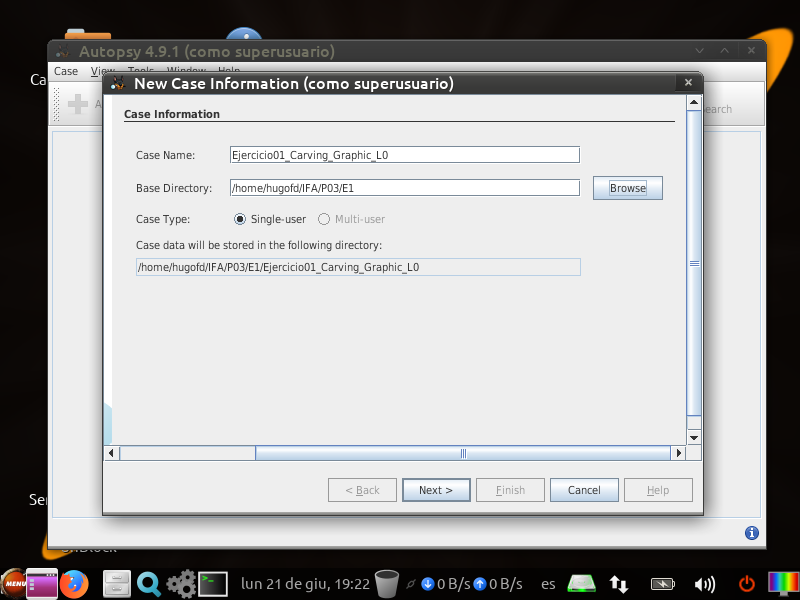
\includegraphics[scale=0.7]{e1-1.png}
\end{figure}

\begin{figure}[H]
  \caption{Ejercicio 1: Detalles del examinador}
  \centering
  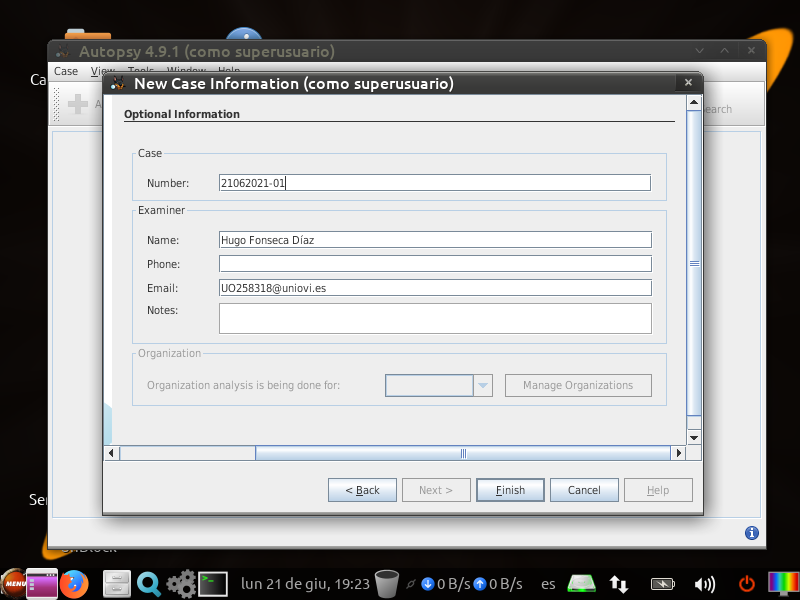
\includegraphics[scale=0.7]{e1-2.png}
\end{figure}

Añadimos la imagen a analizar.

\begin{figure}[H]
  \caption{Ejercicio 1: Selección de la imagen}
  \centering
  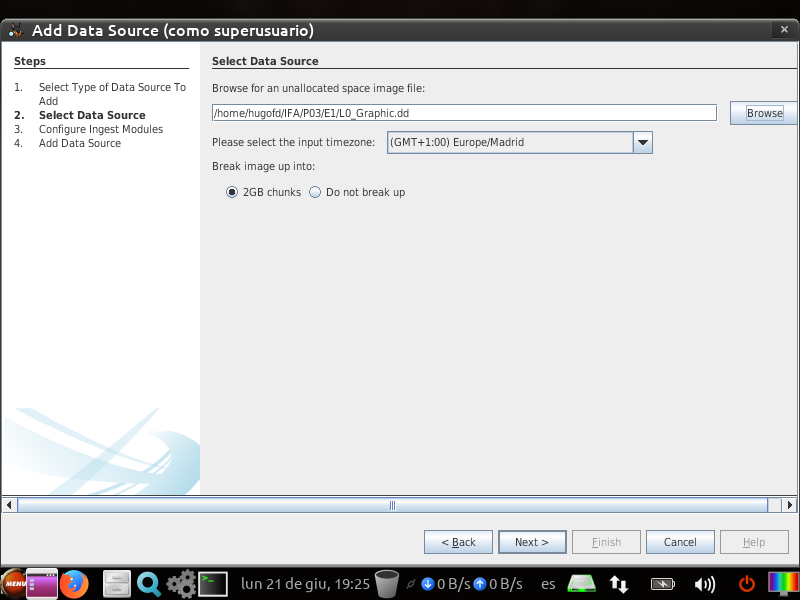
\includegraphics[scale=0.7]{e1-3.png}
\end{figure}

Se seleccionan los módulos de identificación de tipos de fichero, parseador de Exif y \textit{PhotoRec Carver}.

\begin{figure}[H]
  \caption{Ejercicio 1: Selección de módulos}
  \centering
  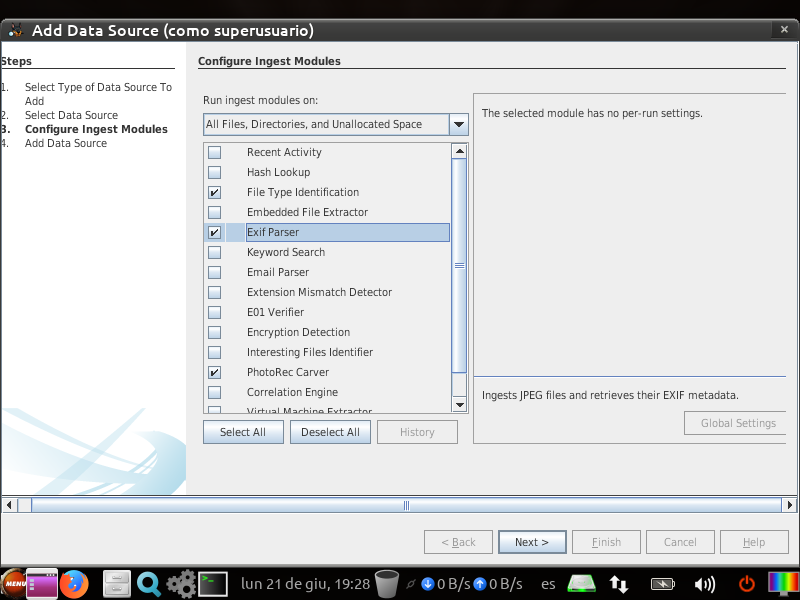
\includegraphics[scale=0.7]{e1-4.png}
\end{figure}

Se ejecuta el análisis y se obtienen los resultados con los que se rellenará la tabla.

\begin{figure}[H]
  \caption{Ejercicio 1: Resultados del análisis}
  \centering
  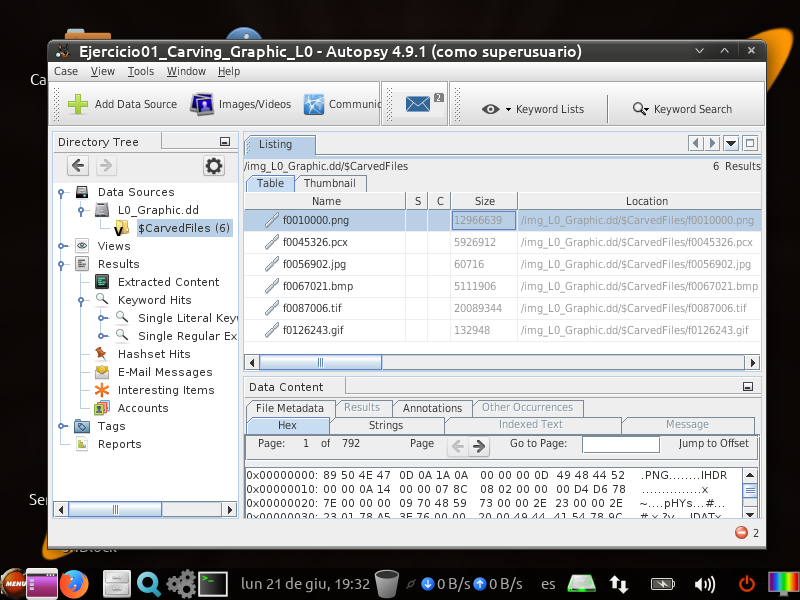
\includegraphics[scale=0.7]{e1-5.png}
\end{figure}

\begin{figure}[H]
  \caption{Ejercicio 1: Imágenes obtenidas}
  \centering
  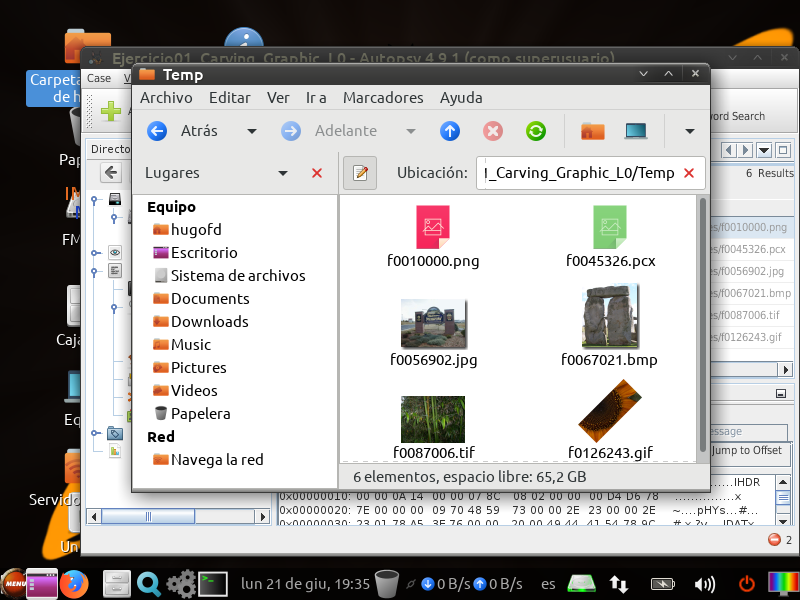
\includegraphics[scale=0.7]{e1-6.png}
\end{figure}

Para abrir el archivo con extensión \textit{pcx} se ha utilizado un visor de imágenes online, al no disponer de uno adecuado en el equipo.

% Ejercicio 2
\section{Ejercicio 2}
Se crea el caso en Autopsy con los datos solicitados.

\begin{figure}[H]
  \caption{Ejercicio 2: Creación del caso}
  \centering
  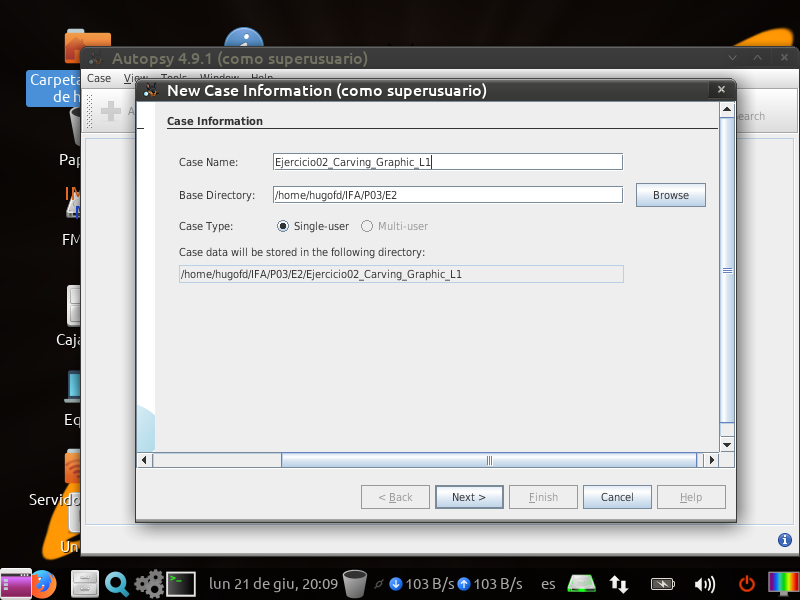
\includegraphics[scale=0.7]{e2-1.png}
\end{figure}

\begin{figure}[H]
  \caption{Ejercicio 2: Detalles del examinador}
  \centering
  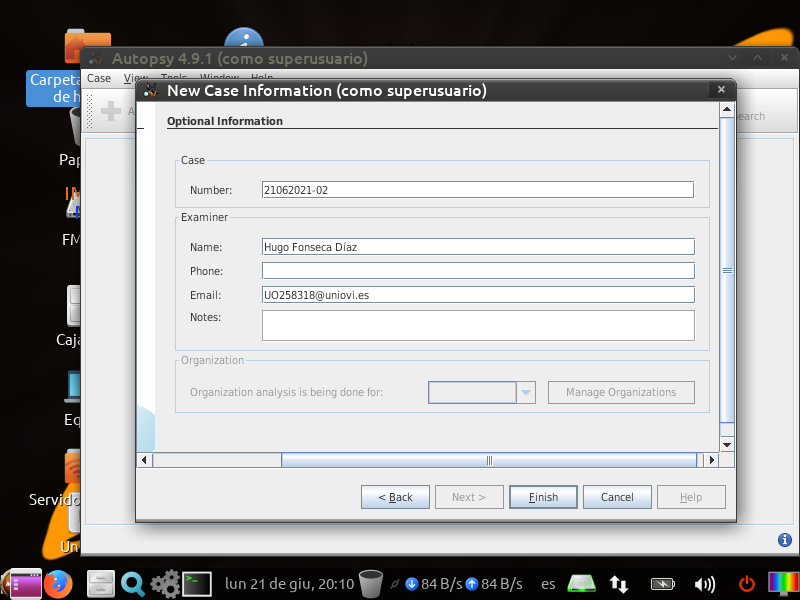
\includegraphics[scale=0.7]{e2-2.png}
\end{figure}

Añadimos la imagen a analizar.

\begin{figure}[H]
  \caption{Ejercicio 2: Selección de la imagen}
  \centering
  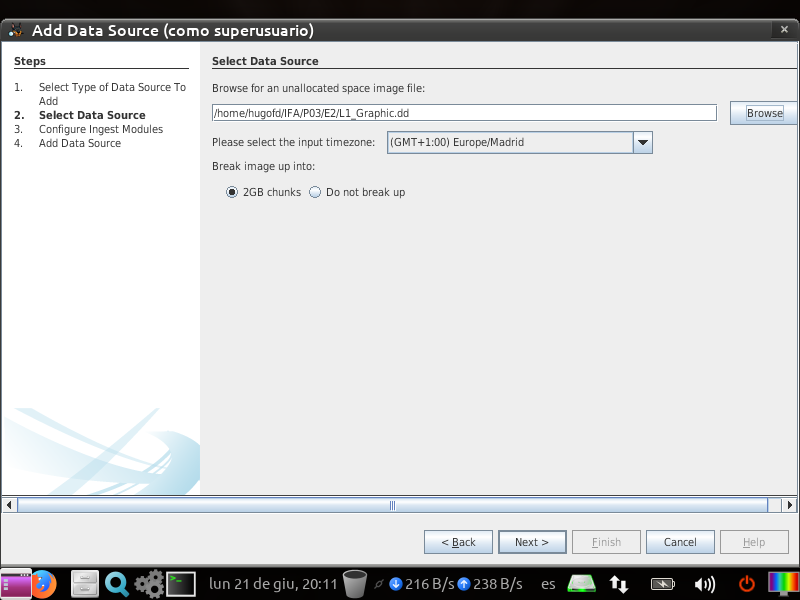
\includegraphics[scale=0.7]{e2-3.png}
\end{figure}

Se seleccionan los módulos de identificación de tipos de fichero, parseador de Exif y \textit{PhotoRec Carver}.

\begin{figure}[H]
  \caption{Ejercicio 2: Selección de módulos}
  \centering
  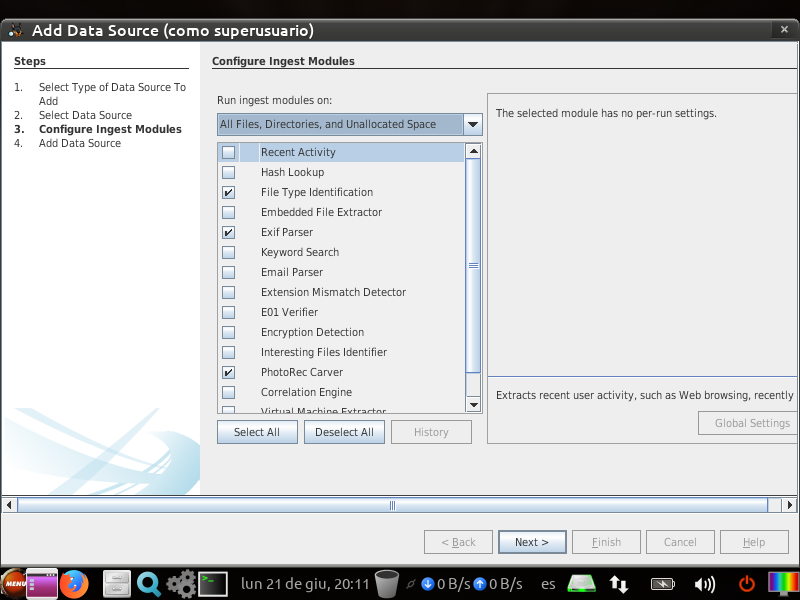
\includegraphics[scale=0.7]{e2-4.png}
\end{figure}

Se ejecuta el análisis y se obtienen los resultados con los que se rellenará la tabla.

\begin{figure}[H]
  \caption{Ejercicio 2: Resultados del análisis}
  \centering
  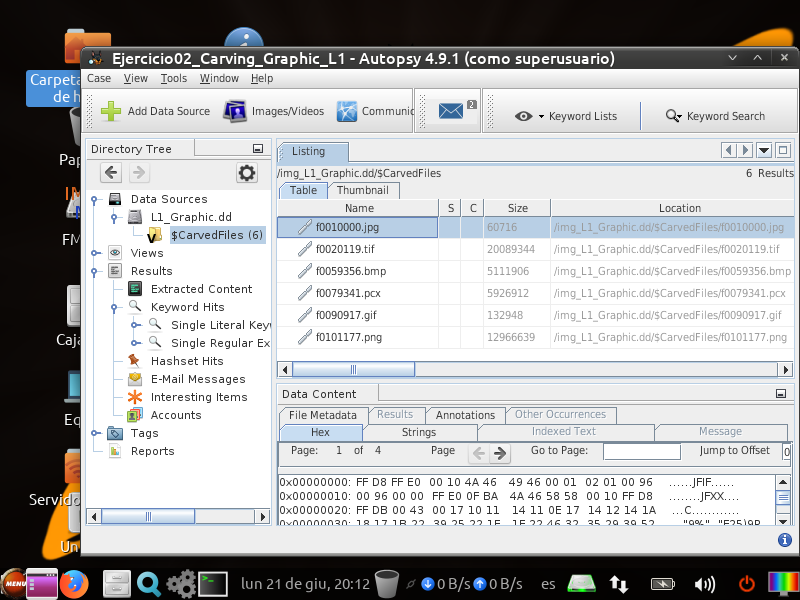
\includegraphics[scale=0.7]{e2-5.png}
\end{figure}

\begin{figure}[H]
  \caption{Ejercicio 2: Imágenes obtenidas}
  \centering
  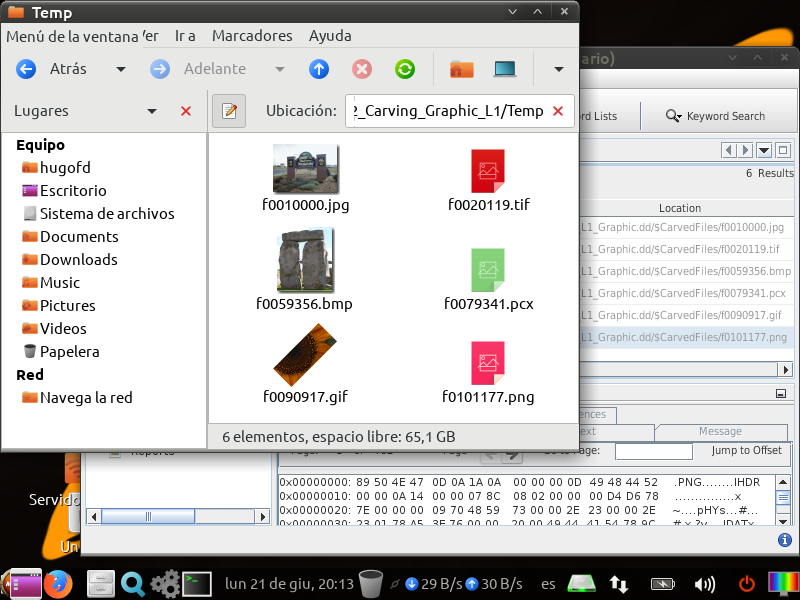
\includegraphics[scale=0.7]{e2-6.png}
\end{figure}

Para abrir el archivo con extensión \textit{pcx} se ha utilizado un visor de imágenes online, al no disponer de uno adecuado en el equipo.



% Bibliografía
\begin{thebibliography}{8}
\end{thebibliography}

\end{document}


